% \documentclass[12pt, twoside]{article}
\usepackage[letterpaper, margin=1in, headsep=0.2in]{geometry}
\setlength{\headheight}{0.6in}
%\usepackage[english]{babel}
\usepackage[utf8]{inputenc}
\usepackage{microtype}
\usepackage{amsmath}
\usepackage{amssymb}
%\usepackage{amsfonts}
\usepackage[nomessages]{fp} %\FPeval{\var-name}{2*sin(pi/6)}
\usepackage{siunitx} %units in math. eg 20\milli\meter
\usepackage{yhmath} % for arcs, overparenth command
\usepackage{tikz} %graphics
\usetikzlibrary{quotes, angles, arrows, arrows.meta}
\usepackage{graphicx} %consider setting \graphicspath{{images/}}
\usepackage{parskip} %no paragraph indent
\usepackage{enumitem}
\usepackage{multicol}
\usepackage{venndiagram}

\usepackage{fancyhdr}
\pagestyle{fancy}
\fancyhf{}
\renewcommand{\headrulewidth}{0pt} % disable the underline of the header
\raggedbottom
\hfuzz=2mm %suppresses overfull box warnings

\usepackage{hyperref}

\fancyhead[LE]{\thepage}
\fancyhead[RO]{\thepage \\ Name: \hspace{4cm} \,\\}
\fancyhead[LO]{BECA / Dr. Huson / Geometry\\*  Unit 2: Angles\\* 11 October 2022}

\begin{document}

\subsubsection*{2.4 Homework: Modeling with algebra, ``Do Not Solve!''}
\begin{enumerate}
\item The ray $\overrightarrow{KM}$ bisects $\angle JKL$. Given m$\angle JKM = 4x-20$ and \\m$\angle MKL = 3x+4$. Identify the true statement(s).
  \begin{multicols}{2}
    \begin{enumerate}
      \item $\angle JKM$ and $\angle MKL$ are a linear pair\\
      $(4x-20) + (3x+4)=180^\circ$
      \item $\angle JKM$, $\angle MKL$ are adjacent and\\
      $4x-20 =90^\circ$
      \item $\angle JKM \cong \angle MKL$\\
      $4x-20 = 3x+4$
   \end{enumerate}
   \begin{center}
     \begin{tikzpicture}[scale=0.6, rotate=-10]
       \draw[<->, thick] (160:5)node[below left]{$J$} 
       --(0,0)node[below left]{$K$}
       --(10:5)node[above right]{$L$};
       \draw[->, thick] (0,0)--(90:5)node[below left]{$M$};
     \end{tikzpicture}
   \end{center}
 \end{multicols}
 
\item The ray $\overrightarrow{BD}$ bisects $\angle ABC$. m$\angle ABD=3x+1$, m$\angle DBC=5x-25$. Find m$\angle ABC$.\vspace{0.5cm}
  \begin{flushright}
  \begin{tikzpicture}
    \draw[<->, thick] (100:4)--(0,0)--(20:5);
    \draw[->, thick] (0,0)--(60:4);
    \draw[fill] (100:3) circle [radius=0.05] node[left]{$A$};
    \draw[fill] (60:3) circle [radius=0.05] node[below right]{$D$};
    \draw[fill] (0,0) circle [radius=0.05] node[below]{$B$};
    \draw[fill] (20:4) circle [radius=0.05] node[below]{$C$};
    \node at (1.5,1){$5x-25$};
    \node at (0.4,2){$3x+1$};
  \end{tikzpicture}
  \end{flushright} \vfill

\item Given the situation in the diagram, answer each question. Circle True or False. \vspace{0.25cm}
  \begin{center}
  \begin{tikzpicture}[scale=0.8, rotate=180]
    \draw[->, thick] (0,0)--(50:3);
    \draw[<->, thick] (-5,.5)--(5,-.5);
    \draw[->, thick] (0,0)--(-1.2,3);
    \draw[fill] (-1,2.5) circle [radius=0.05] node[left ]{$S$};
    \draw[fill] (50:2) circle [radius=0.05] node[above left ]{$T$};
    \draw[fill] (0,0) circle [radius=0.05] node[above right]{$P$};
    \draw[fill] (4,-0.4) circle [radius=0.05] node[below]{$U$};
    \draw[fill] (-4,0.4) circle [radius=0.05] node[below]{$R$};
  \end{tikzpicture}
  \end{center}
  \begin{enumerate}
    \item True or False: $\overrightarrow{RP}$ and $\overrightarrow{UP}$ are opposite rays.
    \item True or False: $\angle TPR$ is supplementary to $\angle TPU$.
    \item True or False: $\angle RPS$ and $\angle TPS$ are complementary angles.
    \item True or False: $\angle RPS$ and $\angle TPU$ are vertical angles.
  \end{enumerate}

\newpage
\subsubsection*{Do Not Solve!}
\emph{Model the situation with an equation. Circle where it states what to solve for.} 
\item Two lines intersect making four angles: $\angle 1$, $\angle 2$, $\angle 3$, and $\angle 4$. Given that m$\angle 1= 4x+30$ and m$\angle 2=8x-10$. Find $x$.
  \begin{flushright}
  \begin{tikzpicture}[scale=0.5, rotate=-10]
    \draw[<->, thick] (0,-1.5)--(10,1.5);
    \draw[<->, thick] (2,2)--(7,-2);
    \node at (3,.4){1};
    \node at (6,-.6){3};
    \node at (5,1){2};
    \node at (4,-1){4};
  \end{tikzpicture}
  \end{flushright}
  
\item In the diagram below $\angle AOB = 30^\circ$ and $\angle COB = 5x+10$. Find $x$. \vspace{0.25cm}
  \begin{flushright}
  \begin{tikzpicture}[scale=0.7, rotate=20]
    \draw[<->, thick] (-25:5)--(0,0)--(155:5);
    \draw[<->, thick] (-5,0)--(5,0);
    \draw[->, thick] (0,0)--(0,4);
    \draw (0,0)++(0.3,0)--++(0,0.3)--+(-0.3,0);
    \draw[fill] (155:3) circle [radius=0.05] node[below left]{$B$};
    \draw[fill] (-4,0) circle [radius=0.05] node[below]{$A$}; 
    \draw[fill] (0,0) circle [radius=0.05] node[below]{$O$};
    \draw[fill] (0,3) circle [radius=0.05] node[left]{$C$};
    \draw[fill] (4,0) circle [radius=0.05] node[below]{$D$};
    \draw[fill] (-25:2) circle [radius=0.05] node[below]{$E$};
  \end{tikzpicture}
  \end{flushright}
    
\item Given that m$\angle 2= 5x+30$ and m$\angle 4=7x-10$ as shown in the diagram, find m$\angle 2$.
  \begin{flushright}
  \begin{tikzpicture}[scale=0.5, rotate=-30]
    \draw[<->, thick] (0,-1.5)--(10,1.5);
    \draw[<->, thick] (2,2)--(7,-2);
    \node at (3,.4){1};
    \node at (6,-.6){3};
    \node at (5,1){2};
    \node at (4,-1){4};
  \end{tikzpicture}
  \end{flushright}

\item In the diagram below $\angle DOE = 60^\circ$ and $\angle DOB = 13x-10$. Find $x$. \vspace{0.25cm}
  \begin{flushright}
  \begin{tikzpicture}[scale=0.7, rotate=-20]
    \draw[<->, thick] (-55:3)--(0,0)--(125:4);
    \draw[<->, thick] (-5,0)--(5,0);
    \draw[->, thick] (0,0)--(0,4);
    \draw (0,0)++(0.3,0)--++(0,0.3)--+(-0.3,0);
    \draw[fill] (125:3) circle [radius=0.05] node[below left]{$B$};
    \draw[fill] (-4,0) circle [radius=0.05] node[below]{$A$}; 
    \draw[fill] (0,0) circle [radius=0.05] node[below left]{$O$};
    \draw[fill] (0,3) circle [radius=0.05] node[left]{$C$};
    \draw[fill] (4,0) circle [radius=0.05] node[below]{$D$};
    \draw[fill] (-55:2) circle [radius=0.05] node[left]{$E$};
  \end{tikzpicture}
  \end{flushright}


\end{enumerate}
\end{document}